\section{分层确定性钱包 (BIP32, BIP44)}

在遵循中本聪的每次交易都使用新地址的建议时,为了防止每次交易后都需要对新生成的公私钥进行备份,
钱包客户端需要维护一个预留的密钥池. 这种方式给用户在不同客户端之间进行切换, 以及钱包对用户私钥的管理带来了困难:
在切换时,用户需要导出导入所有相关地址的私钥,并且不能在不同的系统上同时使用钱包.
分层确定性钱包从根节点确定性派生密钥树的方法很好地解决了这个问题.

分层确定性钱包是由Pieter Wuille在2012年于BIP32中提出的.
分层确定性钱包中, 从根节点出发按照层级结构以一种确定性的方式从parent key 派生 child key,
从而建立起一棵由根节点完全派生的树.因此,当用户在两个支持该协议的不同客户端之间进行切换时,密钥的导入、
导出只需要复制根节点(主密钥)的信息,钱包可以根据根节点和该协议规定的派生方法确定性地派生出整棵密钥树.
因此,用户可以方便地在不同客户端之间切换,钱包也可以依据密钥的派生层级对密钥进行逻辑上的分层管理.
  
此外,该协议允许子私钥和子公钥的派生过程相互独立,
即父私钥可以派生出子私钥和子公钥,而父公钥只能派生出子公钥.
这种机制允许在不安全的环境中,在没有父私钥访问权限的情况下,
依然可以进行子公钥的派生,从而防止父私钥的泄露.
同时,钱包的树状结构有助于用户对访问权限进行选择性的共享
(这取决于共享的密钥所处的层级,以及共享的是私钥还是公钥).  

BIP32着重讲述分层确定性钱包的原理,对于客户端如何实现并没有做严格的限制,
因此,2014年,Marek Palatinus和Pavol Rusnak 
提出了BIP44, 旨在BIP32的基础上对钱包具体的实现方式,不同层级的逻辑含义进行了规定.

\subsection{BIP32: 分层确定性钱包的密钥派生}

在使用该协议从父节点派生子节点时,实际上使用的是512比特的扩展密钥$(k,c)/(K,c)$,
其中$k$代表私钥, $K$代表公钥, $c$则称为链码(Chain Code),作为额外的256比特的熵.
对于扩展公私钥对,其中只有公私钥部分不同,链码是相同的.
 
每一个扩展密钥至多可以有$2^{31}$个平凡子密钥(Normal Child Key)和$2^{31}$个增强子密钥(Hardened Child Key), 
平凡子密钥对应的索引(Index)从0到$2^{31}-1$, 增强子密钥的索引则从$2^{31}$ 到$2^{32}-1$.
为便于表示, 我们用$i_H$表示增强子密钥的索引 $i+2^{31}$. 增强子密钥的引入是为了增强整个方案的安全性,
具体原理在Section~\ref{sec-security}~一节会详细介绍. 
下面首先介绍从父私钥(Private Parent Key)到子私钥(Private Child Key)的派生过程.

%\subsubsection{父私钥派生子私钥}
 
%\begin{figure}[h]
%\centering
%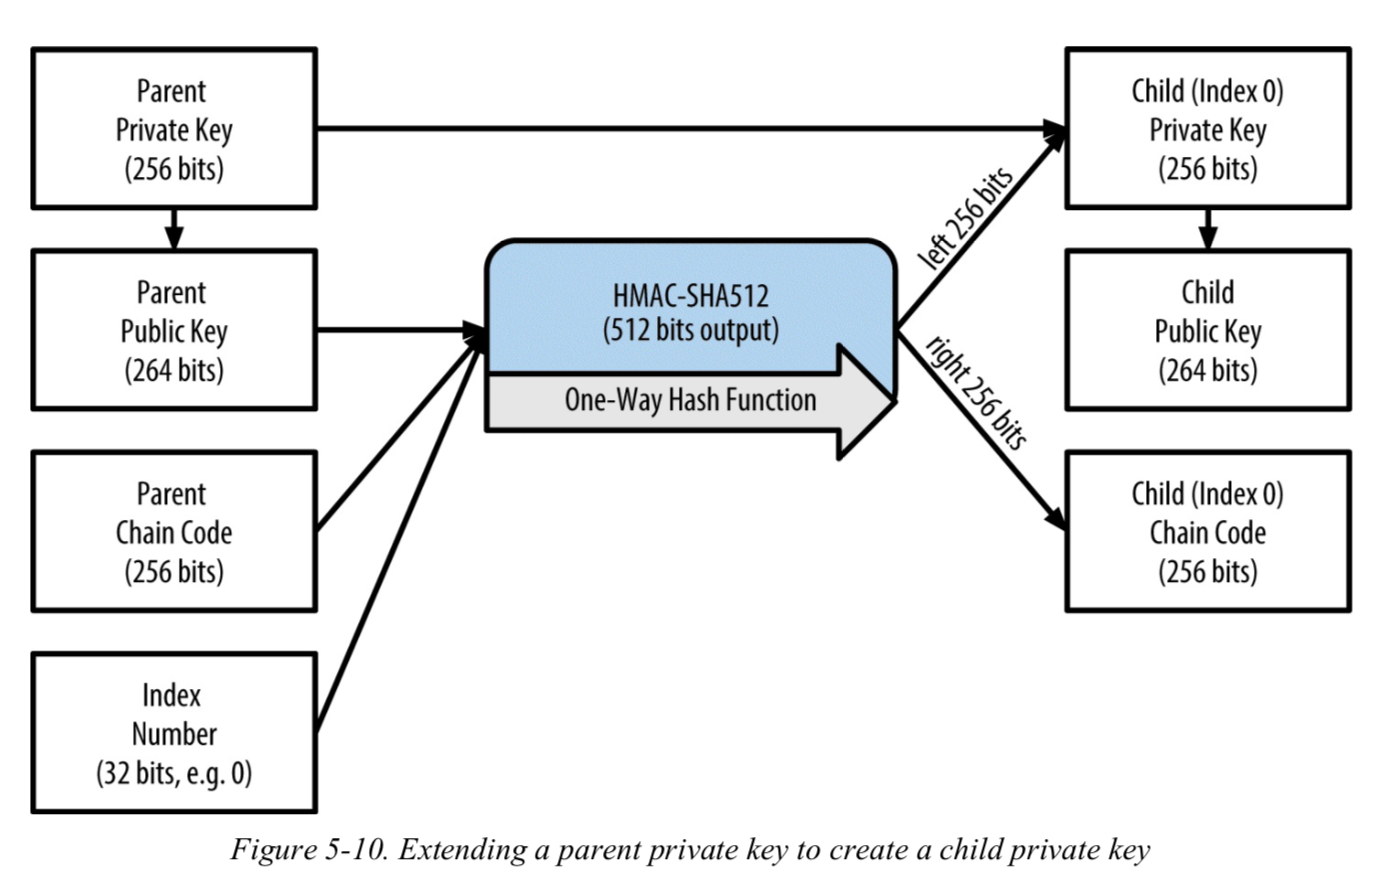
\includegraphics[width=.7\textwidth]{./CKDpriv.png}
%\caption{Normal child 的派生过程(图片来自《Master Bitcoin》)}\label{fig-parsesig}
%\end{figure}
 
\begin{algorithm}[h]\footnotesize
\caption{子私钥派生算法}\label{algo-drc-priv}
  	\begin{algorithmic}[1]
	    \STATE 函数 $\textsf{CKDpriv}((k_{par}, c_{par}), i) \rightarrow (k_i, c_i)$ 从父扩展私钥计算子扩展私钥:
		\STATE 判断索引$i$是否大于等于$2^{31}$, 也即判断子密钥的类型
		\IF {hardened child}
			\STATE let $I = \textsf{HMAC-SHA512}(Key = c_{par}, Data = 0x00 || ser_{256}(k_{par}) || ser_{32}(i))$
		\ELSE
			\STATE let $I = \textsf{HMAC-SHA512}(Key = c_{par}, Data = ser_P(k_{par}G) || ser_{32}(i))$
		\ENDIF
		\STATE 拆分$I$为两个32字节: $I_L || I_R = I, I_L = I[0,\cdots,31], I_R = I[32, \cdots, 63]$.
		\STATE 子私钥 $k_i = parse_{256}(I_L) + k_{par} \mod n $, 对应的链码$c_i = I_R$.
		\STATE 如果$parse256(I_L) \geq n$或者$k_i = 0$, 则计算结果不合法,此时递增$i$并重新计算.
    \end{algorithmic}
\end{algorithm}

在上述算法的第4步中, $Data$参数中的前缀$0x00$字节将私钥补齐为33个字节,与压缩形式的公钥(第6步)一样长.
而第10步中,计算结果不合法发生的概率大概为$1/2^{127}$.
根据上述算法也可以发现,派生增强子密钥和平凡子密钥时$\textsf{HMAC-SHA512}$计算的密钥均为父链码$c_{par}$,
然而输入参数$Data$的构造方式不同.
派生平凡子私钥(Private Normal Child Key)时, $Data = ser_P(k_{par}G) || ser_{32}(i))$,
而在派生增强子私钥(Private Hardened Child Key)时, $Data = 0x00 || ser_{256}(k_{par}) || ser_{32}(i))$.
可以注意到平凡子私钥的派生只需要父公钥$k_{par}G$, 则增强子私钥的派生则需要父私钥$k_{par}$,
这也就限定了增强子密钥只能通过父私钥进行派生(无论是计算增强子私钥还是增强子公钥).

%\begin{figure}[h]
%\centering
%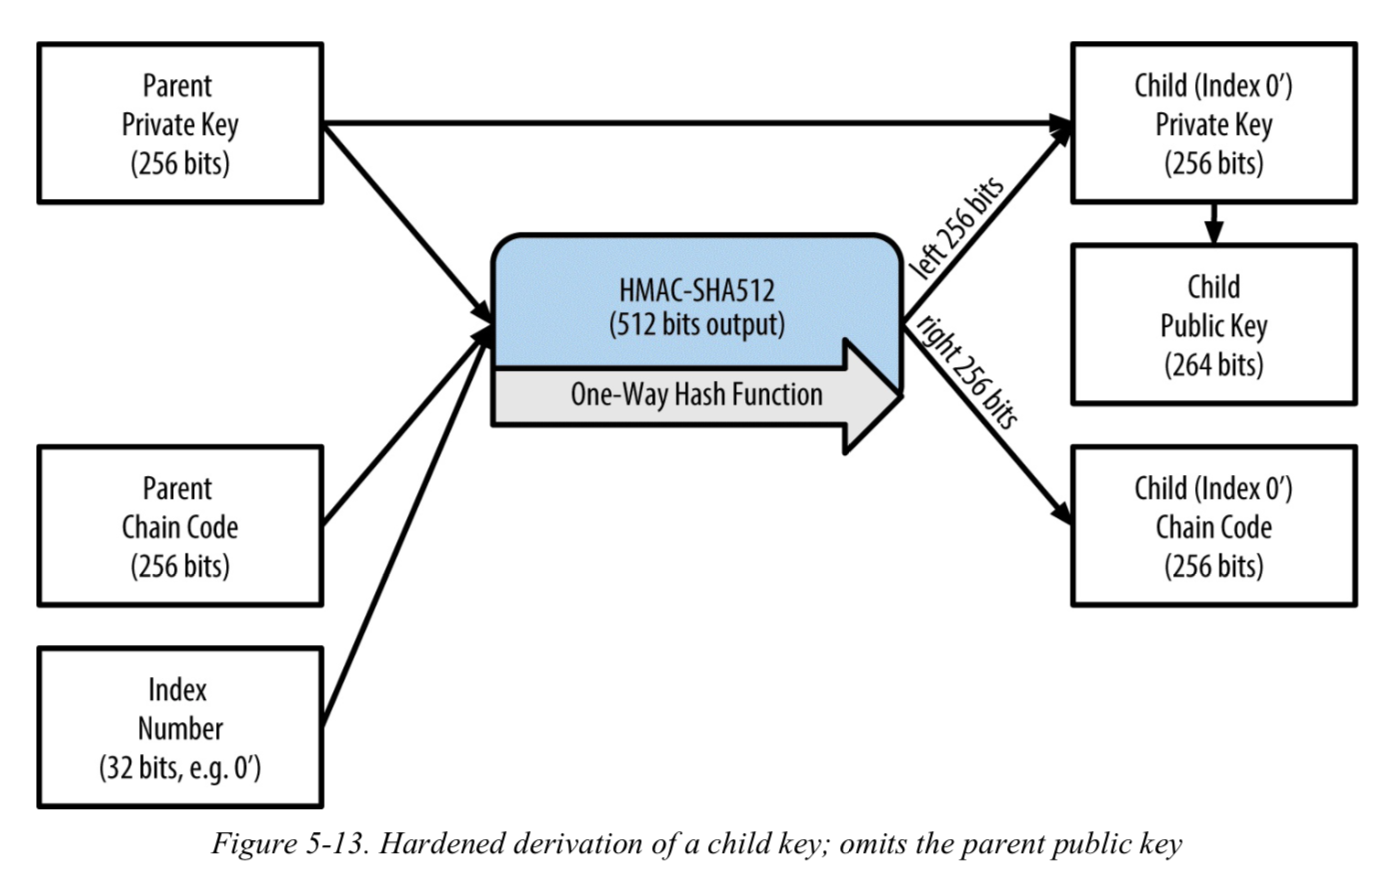
\includegraphics[width=.7\textwidth]{./CKDpriv2.png}
%\caption{Hardened child 的派生过程(图片来自《Master Bitcoin》)}\label{fig-parsesig}
%\end{figure}

%\subsubsection{父公钥派生子公钥}

%\begin{figure}[h]
%\centering
%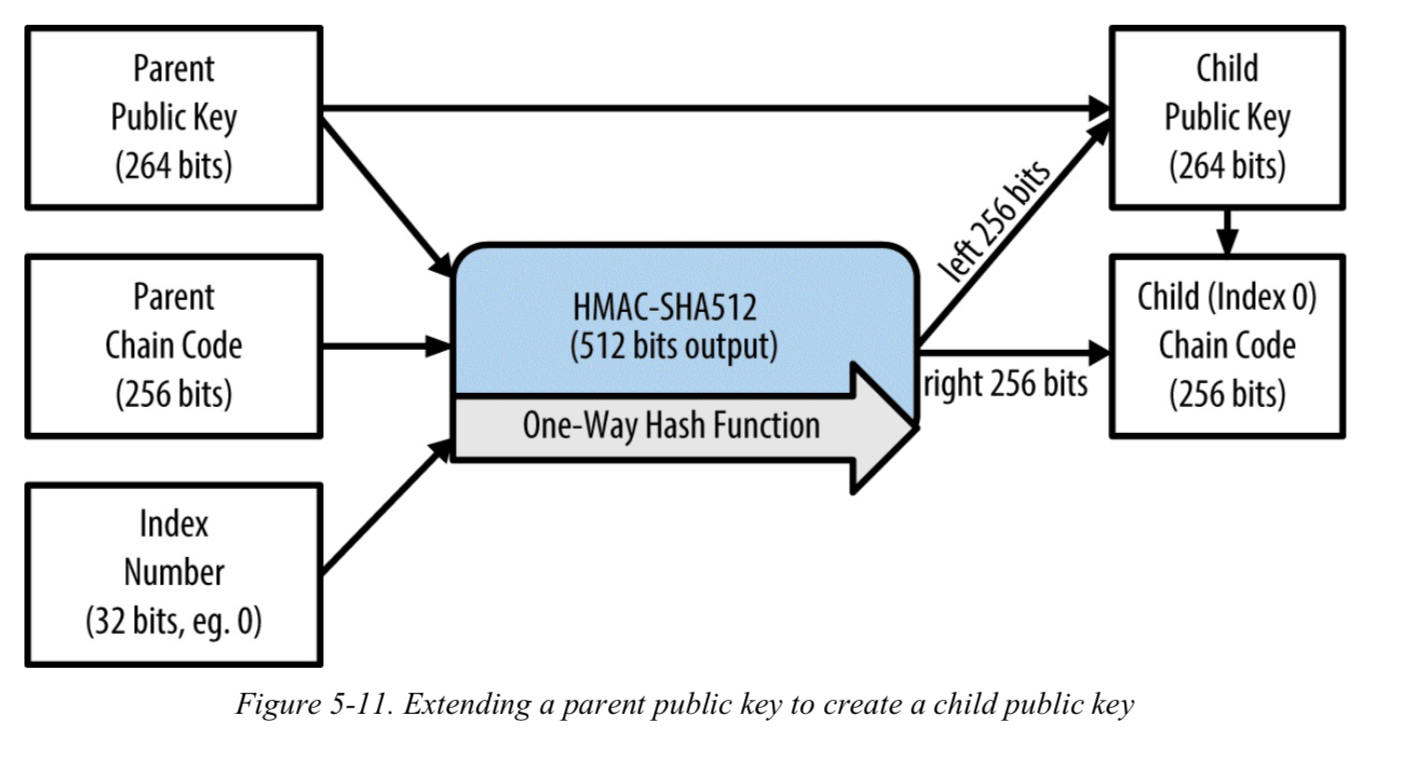
\includegraphics[width=.7\textwidth]{./CKDpub.png}
%\caption{}\label{fig-parsesig}
%\end{figure}

从父公钥派生子公钥的过程在算法~\ref{algo-drc-pub}~中给出,注意该过程只适用于派生平凡子公钥的情形.
从父公钥派生子公钥时, 最终的子公钥$K_i = parse_{256}(I_L) + K_{par}$.

\begin{algorithm}[h]\footnotesize
\caption{子公钥派生算法}\label{algo-drc-pub}
  	\begin{algorithmic}[1]
	    	\STATE 函数$\textsf{CKDpub}((K_{par}, c_{par}), i) \rightarrow (K_i, c_i)$从父扩展公钥计算子扩展公钥
		\STATE 判断索引$i$是否大于等于$2^{31}$, 也即判断子密钥的类型
		\IF {hardened child}
			\STATE return failure  
		\ELSE
			\STATE let $I = \textsf{HMAC-SHA512}(Key = c_{par}, Data = ser_P(K_{par}) || ser_{32}(i))$. 
		\ENDIF
		\STATE 拆分$I$为两个32字节: $I_L || I_R = I, I_L = I[0,\cdots,31], I_R = I[32, \cdots, 63]$.
		\STATE 子公钥$K_i = parse_{256}(I_L) + K_{par}$, 对应的链码为 $c_i = I_R$.
		\STATE 如果$parse_{256}(I_L\geq n)$或者 $K_i$为无穷远点,则递增$i$重新计算
    \end{algorithmic}
\end{algorithm}

椭圆曲线点群上点加法与$\Z_n$上模$n$加法的同态性保证了按照
算法~\ref{algo-drc-pub}~派生而来的子公钥与算法~\ref{algo-drc-priv}~中根据相同索引派生出的子私钥是一一对应的.
这也就是在计算平凡子密钥时, 平凡子公钥和平凡子私钥的派生可以分开独立进行的原因.
记$E(\F_p)$为基于有限域$\F_p$, 基点为$G$, 阶数为$n$的椭圆曲线点群, 
则存在一个从$\Z_n$到$E(\F_p)$的映射$f(x)=xG, x\in\Z_n$,并且该映射$f$是保持加法操作的:
即对于$\Z_n$上的任意值$x$, 都有
$$ f(x+\Delta_x)=f(x)+f(\Delta_x) \Leftrightarrow (x + \Delta_x)G = xG + \Delta_xG, \text{其中}\ \Delta_x \in \Z_n.$$ 
把上式中的$x$当做父私钥, 而$\Delta_x$当做$\textsf{HMAC-SHA512}$输出的$I_L$,
则$f$即为从私钥计算相应公钥的过程.
这也就是说,将私钥$x$先加上一个偏移量$\Delta_x$,再通过$f$变换得到的结果,
与先将私钥$x$和偏移$\Delta_x$映射到公钥,再做加法得到的结果是相同的.


\begin{figure}
\centering
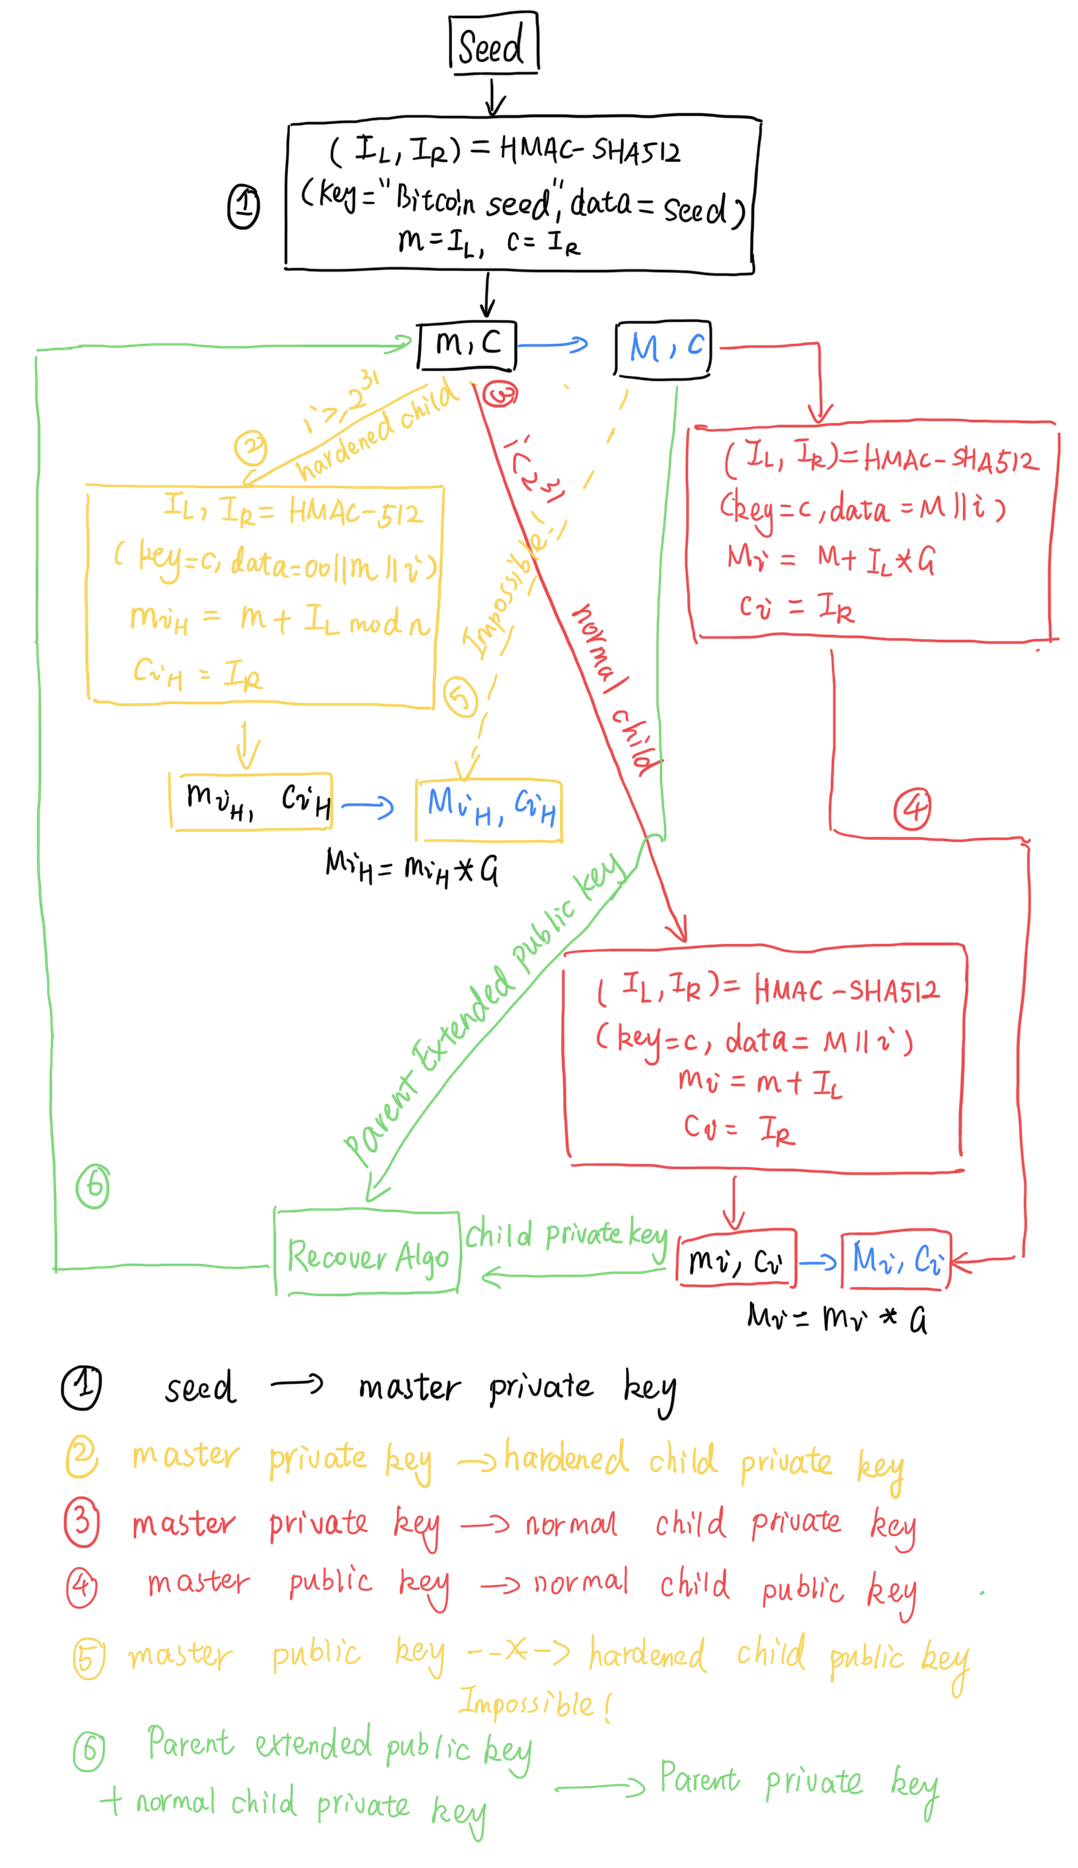
\includegraphics[width=.7\textwidth]{./outline.png}
\caption{分层确定性钱包密钥派生原理}\label{fig-bip32}
\end{figure}


根据算法~\ref{algo-drc-priv}~和算法~\ref{algo-drc-pub}~可知,有两种方式从父私钥派生子公钥.
可以先根据算法~\ref{algo-drc-priv}~从父私钥派生出子私钥然后得到子公钥:
$$k_i, c_i = \textsf{CKDpriv}((k_{par}, c_{par}), i),\ K_i = k_iG.$$
也可以先根据父私钥计算父公钥,然后根据算法~\ref{algo-drc-pub}~得到子公钥
$$K_{par} = k_{par}G,\ K_i, c_i = \textsf{CKDpub}((K_{par}, c_{par}), i).$$ 
如前所述,算法~\ref{algo-drc-pub}~只适用于平凡子密钥派生的情形.

根据算法~\ref{algo-drc-priv}~和算法~\ref{algo-drc-pub}~可知, 可以从一个扩展密钥出发,
逐层派生出一棵密钥树,通常称这个扩展密钥为扩展主密钥.
扩展主密钥通常不是直接生成的,而是从一个可能更短的种子派生而来.
BIP-32中给出了具体的计算步骤.
首先利用密码学安全的的伪随机数发生器(Cryptographically Secure Pseudo-Random Number Generator)生成种子$Seed$.
种子的比特长度通常介于128比特到512比特之间,推荐使用256比特.然后执行如下计算:
$$I = \textsf{HMAC-SHA512}(Key = ``Bitcoin seed", Data = Seed),$$
将$I$划分$I_L = [0,\cdots,31], I_R = [32,\cdots,63]$,
则扩展主私钥为$I_L$, 主链码(Master Chain Code)为$I_R$.
有了扩展主密钥之后,就可以根据算法~\ref{algo-drc-priv}~和算法~\ref{algo-drc-pub}~逐层派生密钥树.
密钥派生的整体结构图参见Figure~\ref{fig-bip32}~,其中绿色表示Recover算法, Section~\ref{sec-security}~中具体阐述.



\subsection{BIP44: 分层确定性钱包的逻辑分层}

为了方便标记和说明, 将$\CKDpriv (\CKDpriv (\CKDpriv (m,3_H),2),5)$记为 $m/3_H/2/5$,
将$\CKDpub (\CKDpub (\CKDpub (M,3),2),5)$记为$M/3/2/5$.其中$m$代表主私钥, $M$代表主公钥.
BIP44对确定性钱包的逻辑层次做了如下限定:
$$m / \text{purpose}' / \text{coin-type}' / \text{account}' / \text{change} / \text{address-index},$$
其中符号$'$代表了这一层使用的是增强子密钥的派生方式. 
purpose字段设定为常量$44‘$,代表了逻辑分层符合BIP44规范;
coin-type字段用于表示不同的数字货币, 从而根据数字货币种类对密钥空间进行划分,
对于一种数字货币而言该字段为一个常量,开发者需要为他们的数字货币申请尚未使用的值;
account字段用于根据不同的用户身份和使用目的对密钥空间进行划分,允许钱包将不同账户隔离开来,
字段值从0 开始递增,在当前账户没有任何交易历史的情况下,钱包软件应当阻止新账户的生成,
并且在用户从外部导入种子后,钱包需要恢复所有已经使用过的账户;
change字段为$0$代表外部的密钥链,也即暴露给其他人用来收款的地址,
值为$1$则代表内部的密钥链,对于外部是不可见的,如用作找零地址等;
address-index字段从0开始连续递增,该索引即为BIP32中定义的用于派生子密钥的索引值.

\begin{table}[h]
\centering
\caption{\textbf{数字货币的密钥分层示例}}
\begin{tabular}{|c|c|c|c|c|}
\hline
\small
Coin &  Account  &   Chain  &  Address &  Path \\\hline
Bitcoin &  first  &  external &  first &  m/44'/0'/0'/0/0 \\\hline
Bitcoin &  second  &  external &  first &  m/44'/0'/1'/0/0 \\\hline
Bitcoin &  first  &  change &  first &  m/44'/0'/0'/1/0 \\\hline
Bitcoin &  first  &  external &  second &  m/44'/0'/0'/0/1 \\\hline
Bitcoin Testnet &  first  &  external &  first &  m/44'/1'/0'/0/0\\\hline
\end{tabular}
\end{table}

前面已经提及到, HD钱包的优势在于将很多私钥的管理简化对种子的管理,尤其是进行导入导出时只需要导出导入种子.
钱包方面需要根据用户导入的种子值,对用户使用过的账户进行恢复.具体步骤如下:
\begin{enumerate}
\item 派生第一个账户节点(index = 0)。
\item 派生该账户的外部链节点。
\item 根据下述的gap limit对外部链进行扫描。
\item 如果该外部链的地址上没有发生过交易,则停止扫描。
\item 反之,递增账户的索引序号,并重复上述步骤1。
\end{enumerate}
Gap limit目前被设置为20,即当扫描到某个账户的外部链中有连续20个没有被使用的地址时,就停止扫描.
该算法有效的前提是,存在账户没有被使用时,钱包需要阻止用户通过递增索引继续生成下一个新账户,
并且在同一个账户下,存在20个连续的地址没有被使用时,阻止用户跨越这些地址生成下一个新地址.

\subsection{安全性分析}\label{sec-security}

分层确定性钱包的密钥派生方案能够保证给定一个公钥$K$,
攻击者计算出相应私钥$k$的难度至少和椭圆曲线点群上的离散对数问题一样难
,这是由基于椭圆曲线的密码学方案所提供的.
通过给定的扩展子私钥$(k_i,c_i)$和索引值$i$恢复父私钥$k_{par}$的难度
至少和攻击\textsf{HMAC-SHA512}一样难,而\textsf{HMAC-SHA512}提供了256比特的安全强度.
判断给定的$N$个(索引, 扩展子私钥)对$(i_j, (k_j, c_j)), 0\leq j \leq N, 2\leq N \leq 2^{32}-1$
是否由同一个扩展父私钥派生而来,至少和攻击\textsf{HMAC-SHA512}一样难,也是不现实的.

给定一个扩展父公钥$(K_{par},c_{par})$ 和一个平凡子公钥$K_i$, 找到该子公钥对应的索引$i$是容易的.
平凡子密钥的索引值$i$的取值范围为$0\leq 0\leq2^{31}-1$,在前述条件下,
可以遍历$i$来重复子公钥的派生的过程,并比较派生出的子公钥是否与给定的子公钥相等.
如果相等,则$i$就是该子公钥对应的索引值.

给定一个扩展父公钥$(K_{par},c_{par})$和平凡子私钥$(k_i)$, 计算父私钥$k_{par}$是容易的.
很容易根据平凡子私钥计算平凡子公钥,则根据前述说明,很容易计算出该子密钥对应的索引值$i$.
由于$I = \textsf{HMAC-SHA512}(Key = c_{par}, Data = ser_P(K_{par}) || ser_{32}(i))$, 
并且有$I_L = I[0,\cdots,31], \ I_R = I[32,\cdots,63]$以及$k_i \equiv parse_{256}(I_L) + k_{par} \mod n$.   
则 $k_{par} \equiv k_i-parse_{256}(I_L)\mod n.$

Listing~\ref{lst-recover}~中的代码展示是前述攻击过程的PoC示例,代码基于分层确定性钱包的Python实现库
bip32utils\footnote{\url{https://github.com/lyndsysimon/bip32utils}}.

\begin{lstlisting}[language=python, caption=基于父扩展公钥和平凡子私钥恢复父私钥的攻击示例, label=lst-recover]
CURVE_GEN  = ecdsa.ecdsa.generator_secp256k1
CURVE_ORDER  = CURVE_GEN.order()
BIP32_HARDEN = 0x80000000 
def recover_parent_privkey(parent_pubkey,child_privkey):
	# traverse all possible non-hardened child index (0~2^31-1) to 
	find the corresponding index of child_privkey
	for i in xrange(0, BIP32_HARDEN +1):
		child=parent_pubkey.CKDpub(i)
		if(child.PublicKey()==child_privkey.PublicKey()):
			break
    # if i is larger than 2^31-1, means that it corresponds to a hardened child, 
    then the recovery is impossible
	if i & BIP32_HARDEN:
		print "can not recover parent private key with a hardened child node"
		return
	# data is composed of public key || i
	data=parent_pubkey.PublicKey()+struct.pack(">L",i)
	(Il,Ir)=parent_pubkey.hmac(data)
	Il_int = string_to_int(Il)
	if Il_int > CURVE_ORDER:
	    return None
	cpk_int=string_to_int(child_privkey.k.to_string())
	# recover parent private key ppk_int from cpk_int= ppk_int + Il_int mod n
	ppk_int=(cpk_int-Il_int)%CURVE_ORDER
	return int_to_string(ppk_int).encode('hex')
\end{lstlisting}

按照BIP32\footnote{
\url{https://github.com/bitcoin/bips/blob/33e040b7bdf5d937599d2401454878d6293476c9/bip-0032.mediawiki\#Test_vector_2}}
测试向量2中给定的seed,
计算出相应路径下的child private/public key,按照上述算法
\ref{lst-recover},通过调用\textsf{recover_parent_privkey(M,m/0)}可成功恢复M的私钥m。

这对于分层确定性钱包的安全性有重要影响,因为这意味着知道一个扩展父公钥和平凡子私钥,
就可以推算出父私钥. 因此管理扩展公钥需要比通常的公钥更为谨慎.
对于采用增强方式派生的密钥则不存在上述问题,因为增强密钥只能通过扩展父私钥派生而来.
这也是在BIP44中规定在purpose, coin-type, account层使用hardened 节点的原因,
以防止这三层上一层的私钥被攻击者按照前述程恢复出来.



